\begin{figure}
\chapter{Risk Analysis}
The Risk Analysis table defines a potential set of risks that our group determined were possible to face, as setbacks to timely progression towards our finished project. For each risk, there are two potential consequences, a probability value 0 to 1, a severity value 0 to 10, an impact value (impact=probability*severity), and potential mitigation strategies.
\newline
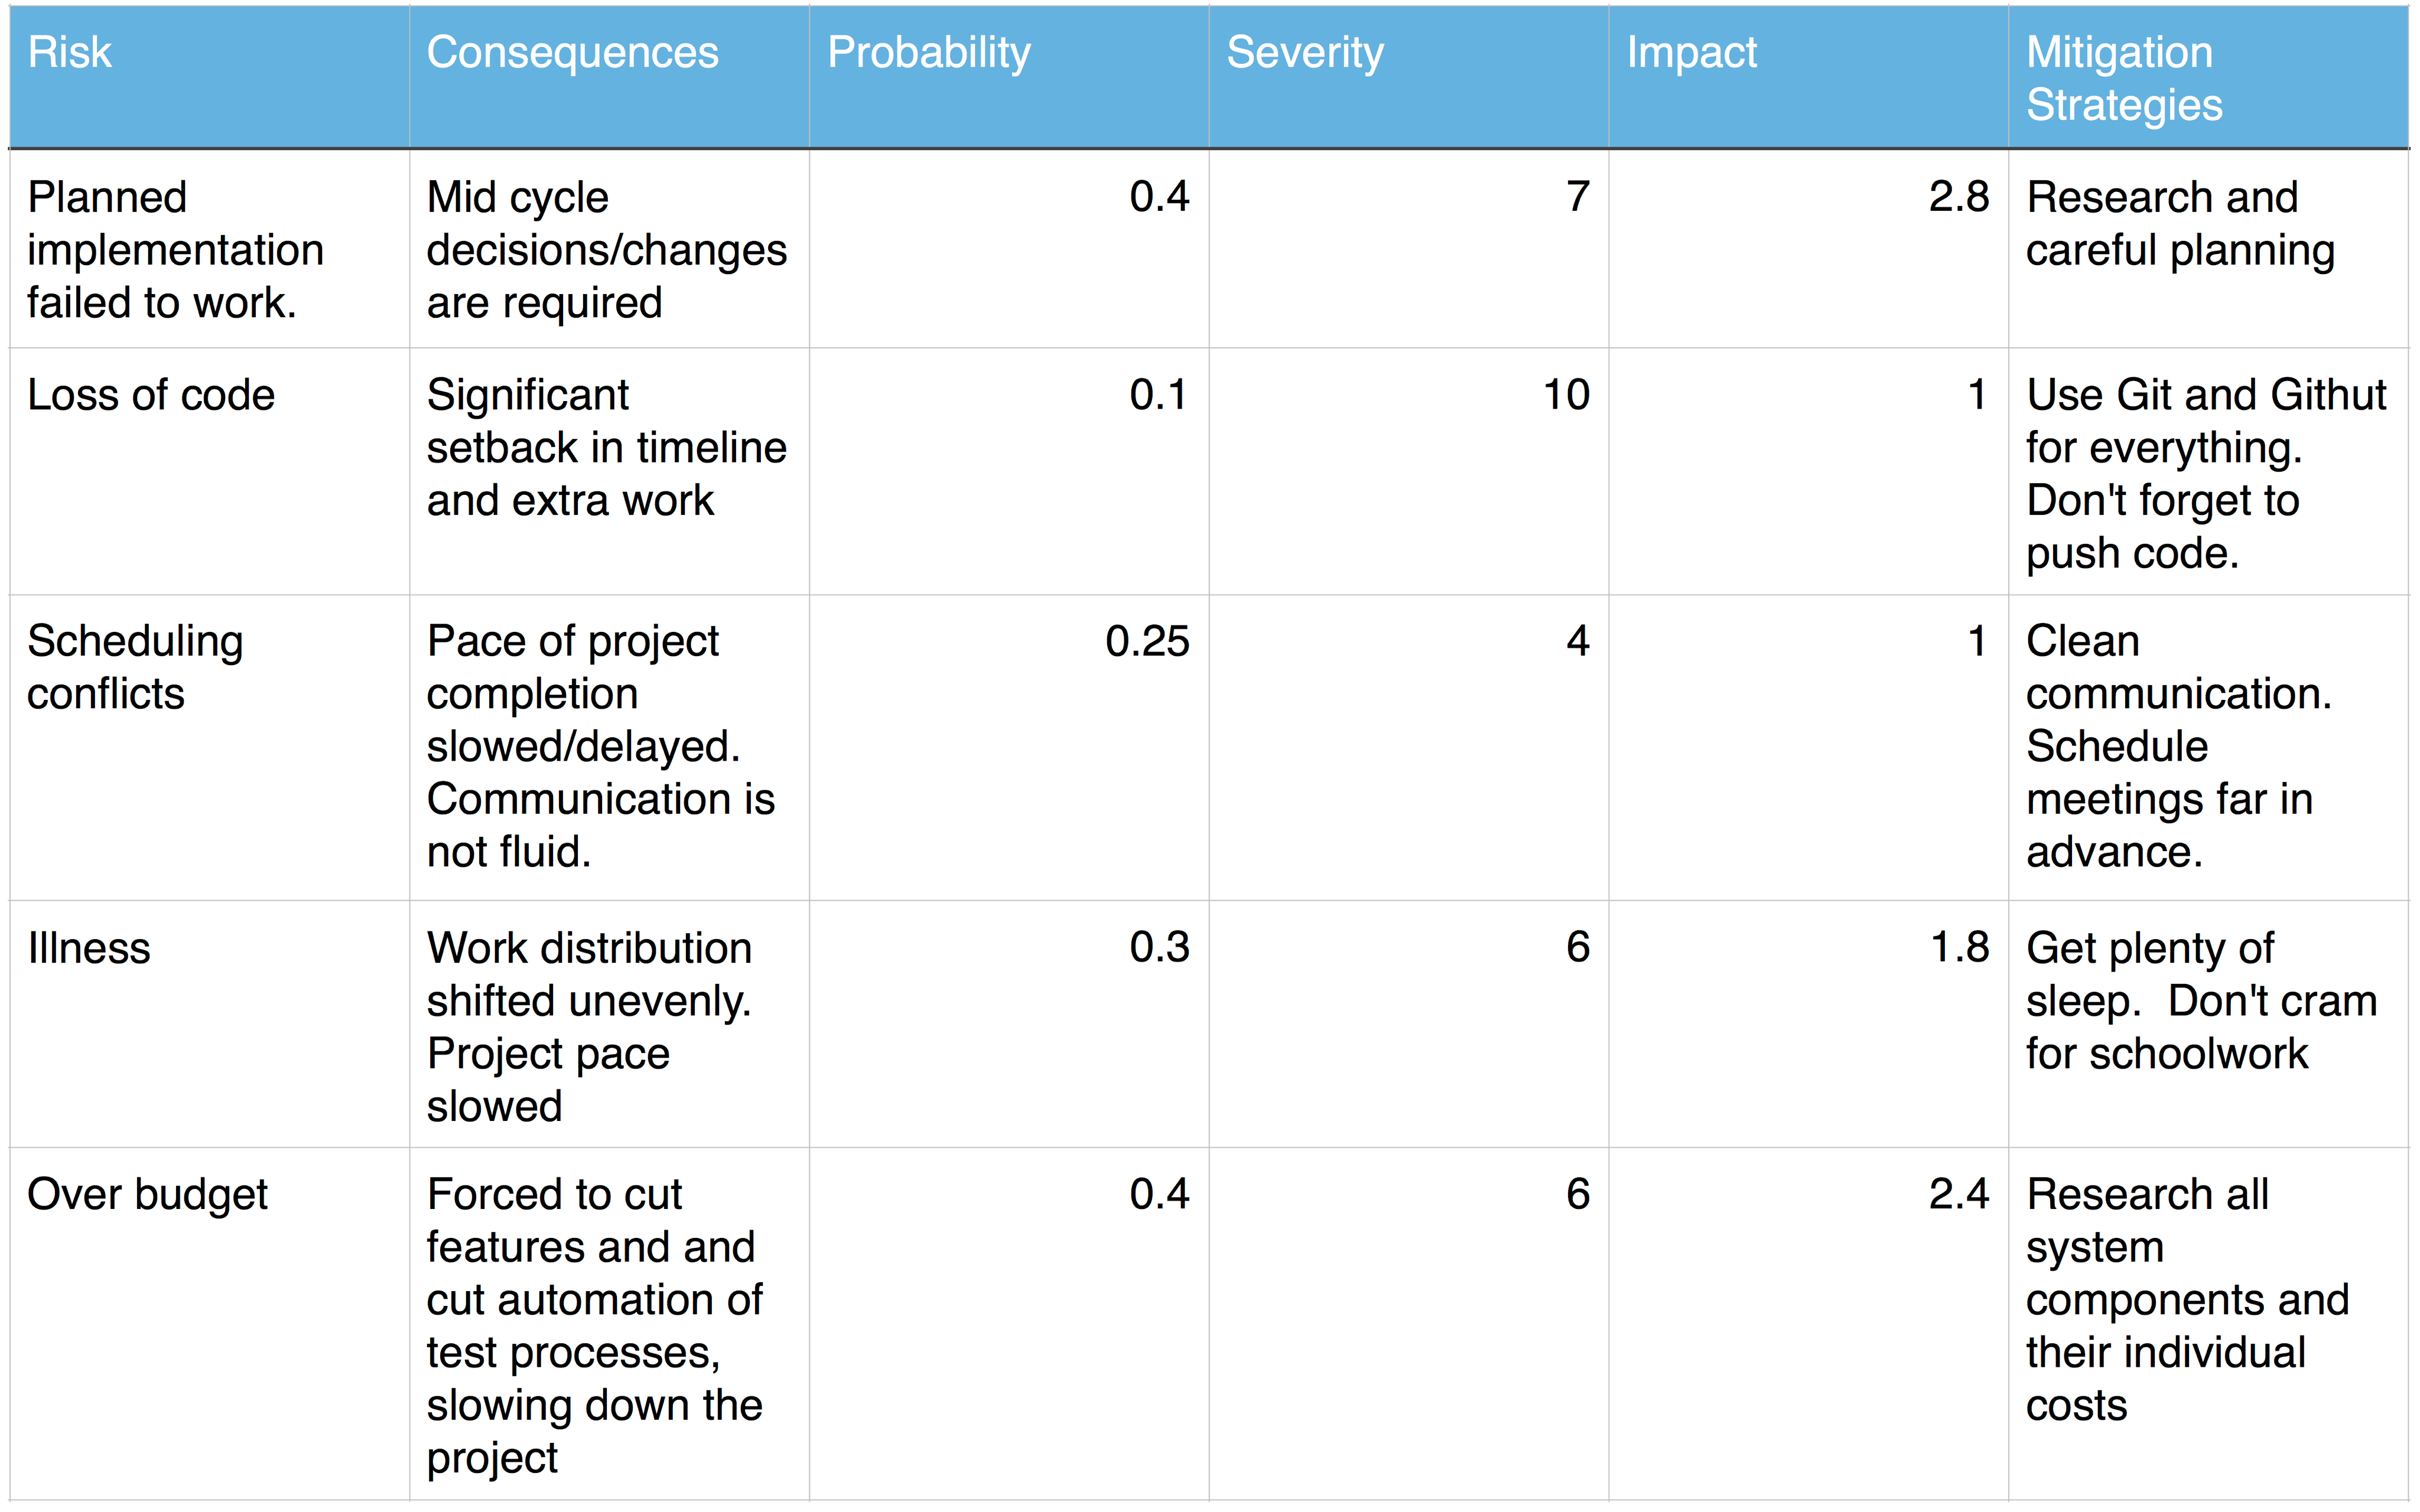
\includegraphics[width=1\textwidth]{images/risk.png}
\caption{Risk Analysis Table}
\par The two most potentially impactful risks are if the planned implementation of the system failed to provide good results, and if the project runs over budget.  By coding in a modular style that provides low coupling, the system can be modified if necessary without having to start from scratch.  Additionally, by buying most line items in the budget up front, we can be sure that the costs do not balloon as the project progresses.
\end{figure}
